\documentclass[11pt]{article}
\usepackage[utf8]{inputenc}
\usepackage{amsmath, amssymb}
\usepackage{graphicx}
\usepackage{hyperref}
\usepackage{geometry}
\usepackage{cite}
\usepackage{listings}
\usepackage{subcaption}

% Geometry settings
\geometry{a4paper, margin=1in}

% Title and author
\title{Planar Cable-Driven Robot}
\author{Arzaq Khan \\
Hamdan Raashid \\
}
\date{\today}

% Code block settings
\lstset{
  basicstyle=\ttfamily\small,
  breaklines=true,
  frame=single,
  numbers=left,
  numberstyle=\tiny,
  xleftmargin=2em,
  language=Python % Change as needed
}

\begin{document}

\maketitle


\section{Introduction}


\subsection{Project Description}
Our project is a planar cable-driven driven that continously tracks and follows objects in real time. If we had been able to
implement everything according to our initial plan, we would have been able to apply the robot in a logistics setting to pick and
place objects. Unfortunately, due to certain problems we encountered, which is discussed in a later section, we were unable to
strictly follow our original plans.

During the planning stage, we aimed to design a planar cable-driven robot that would pick a user selected target and drop off that
target to a user selected location. The user would first select the target in a video feed provided by a staionary camera and the
robot would move the end-effector to where the target is located. Next, a command would be given to the end-effector to switch on the
electromagnet to pick up the target. Then, the user would provide a location to drop off the target using
the same video feed and the robot would drop off the target at said location. 
Although our actual robot is similar to what we had planned initially, there are slight differences.

The main difference between what we built and we had planned lies in the parts we used and the end-effector. We had
planned to use an ESP32, a microcontroller, for its Bluetooth and WiFi features and stepper motors due to their precision.
Unfortunately, we could not get the stepper motors to work. We initially figured that it was a power issue, but even
after connecting the motors to an external power supply, we could not get the motors to move. As for the end-effector,
we could not mount an electromagnet on it due to issues discussed in a subsequent section. To summarize, what we have
is a robot that can continously track and follow objects, but cannot pick them up.

\begin{figure}[h!]
\centering

\begin{subfigure}[b]{0.3\textwidth}
    \centering
    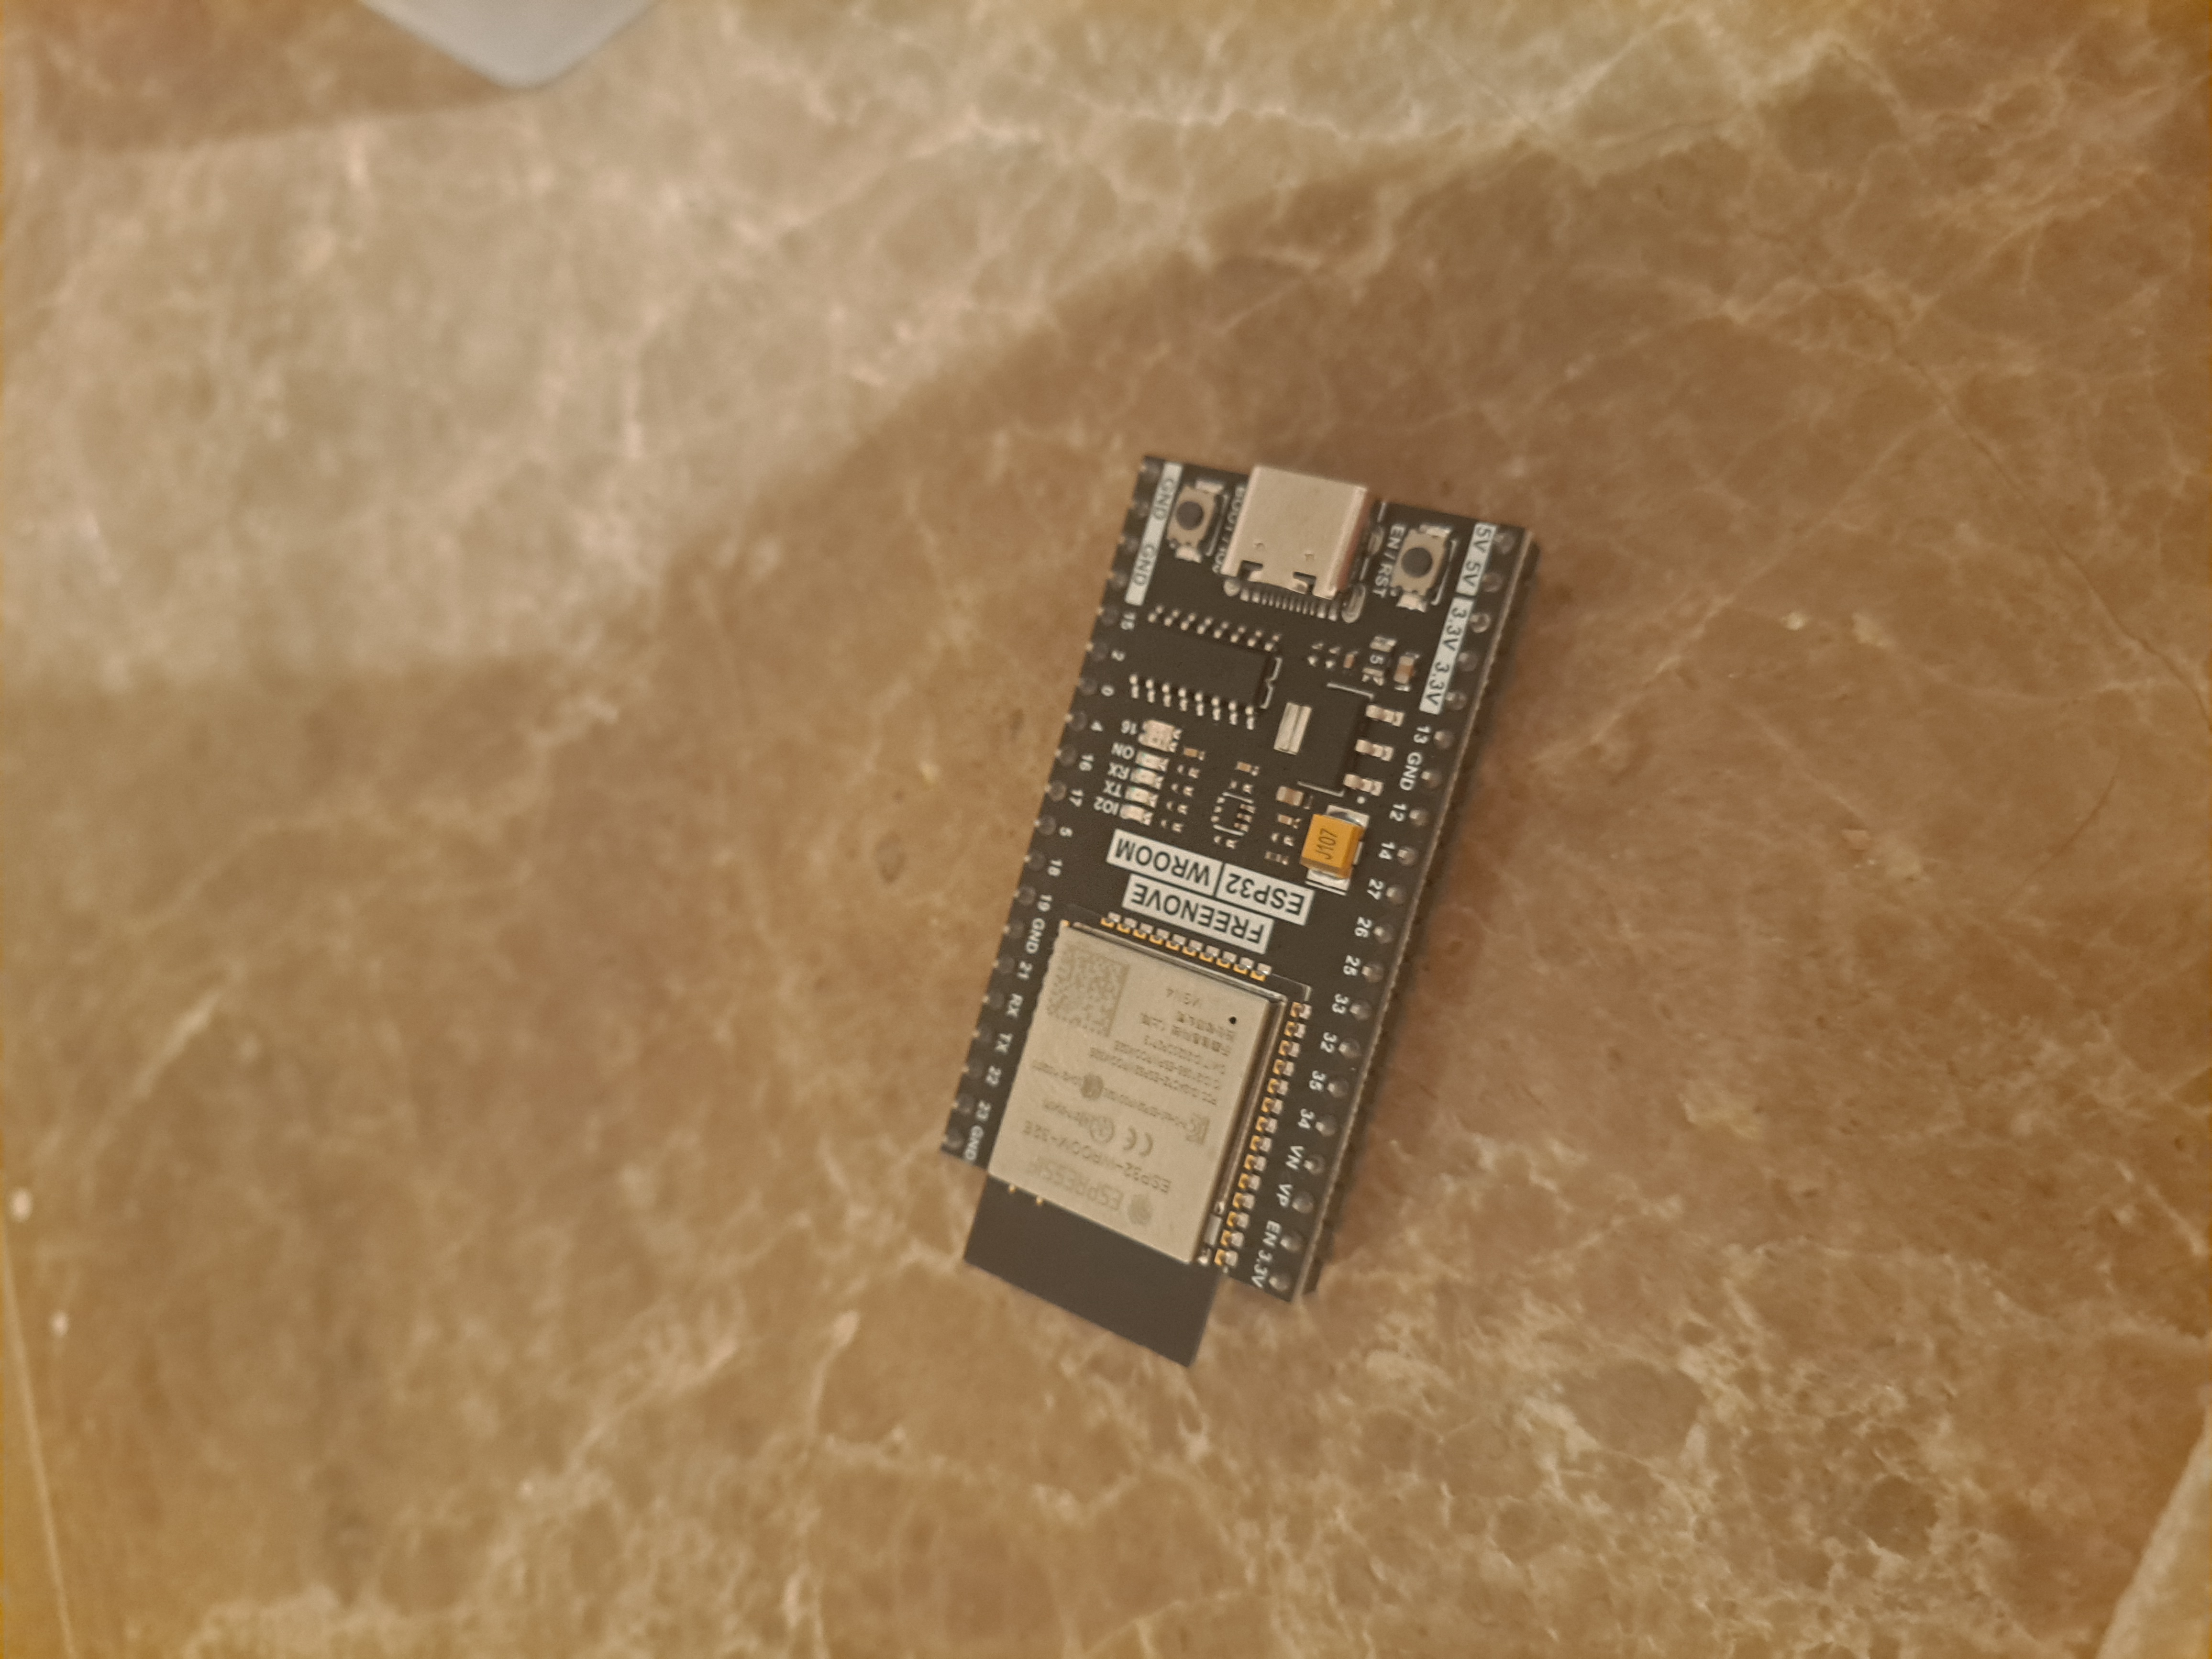
\includegraphics[width=\textwidth]{ESP32Img.jpg}
    \caption{An ESP32 microcontroller.}
    \label{fig:figure1}
\end{subfigure}
\hfill
\begin{subfigure}[b]{0.3\textwidth}
    \centering
    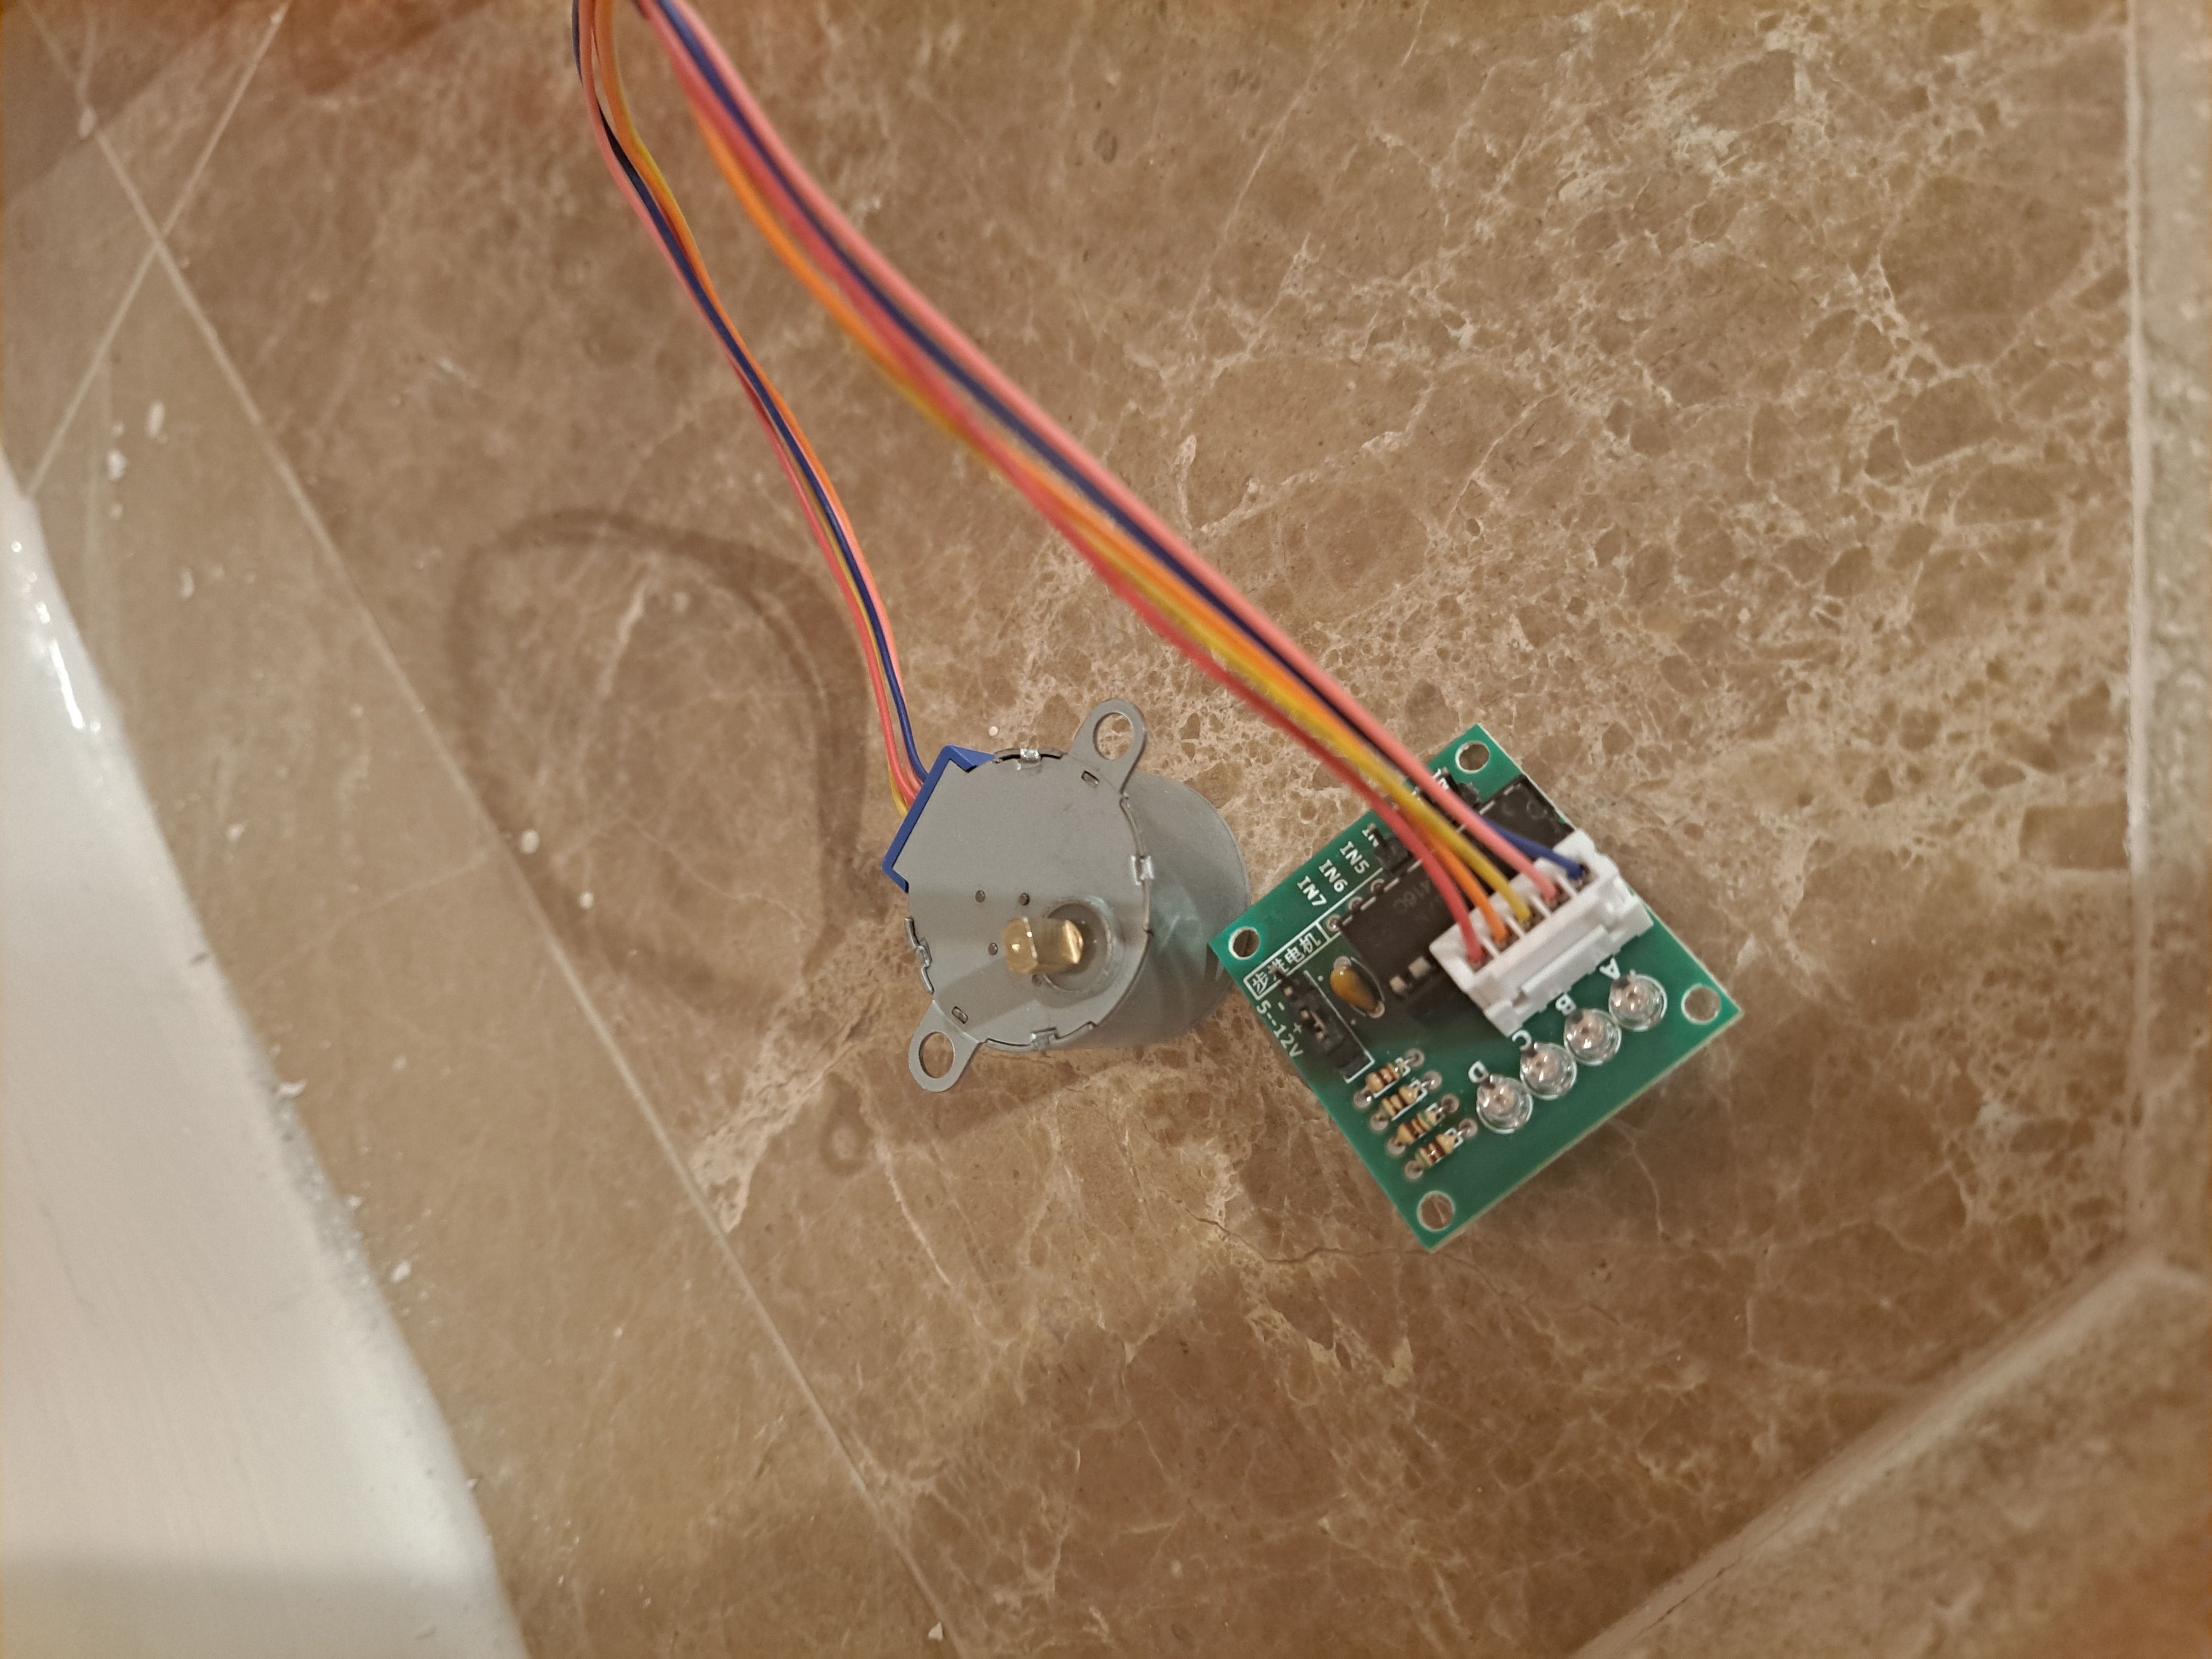
\includegraphics[width=\textwidth]{MotorImg.jpg}
    \caption{A stepper motor.}
    \label{fig:figure2}
\end{subfigure}
\hfill
\begin{subfigure}[b]{0.3\textwidth}
    \centering
    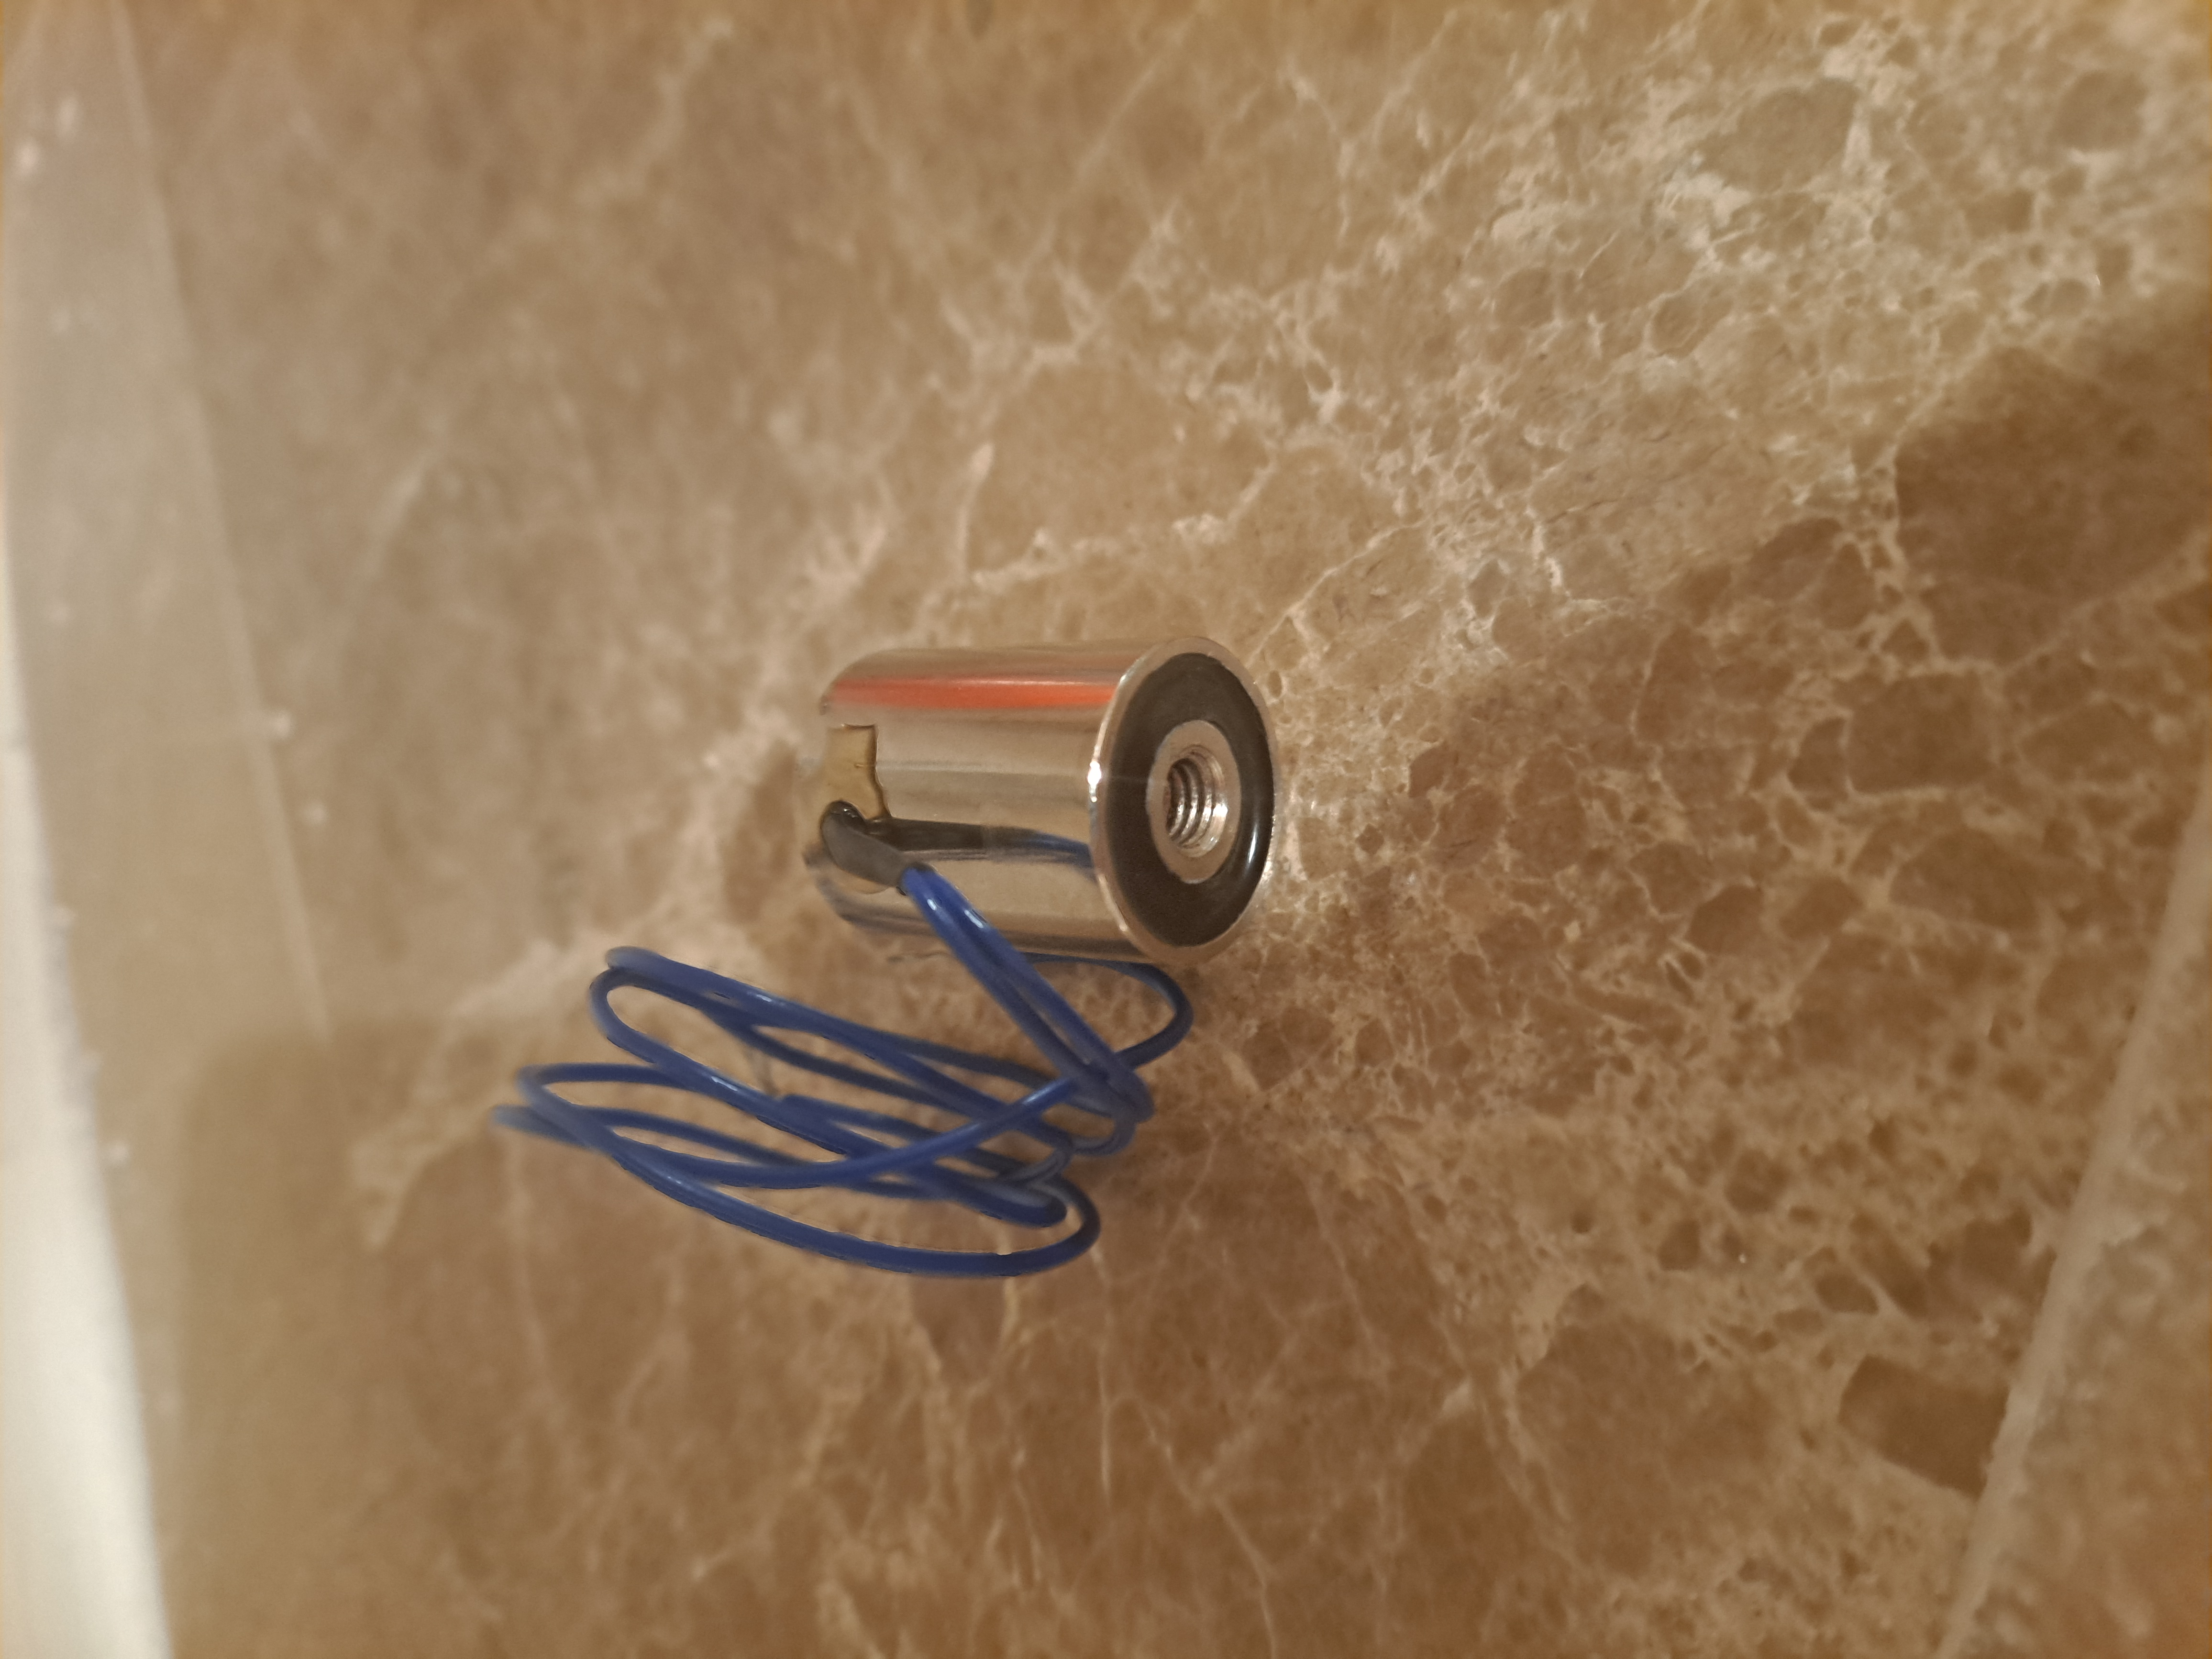
\includegraphics[width=\textwidth]{ElectromagnetImg.jpg}
    \caption{An electromagnet.}
    \label{fig:figure3}
\end{subfigure}

\caption{Three side-by-side figures showing an ESP32, a stepper motor, and an electromagnet.}
\label{fig:side_by_side}
\end{figure}
  


\subsection{Introduction to Cable-Driven Robots}
A cable-driven robot is actuated using cables. The main parts of a cable-driven robot include winches, cables, motors, and 
a mobile platform/end-effector. The active length of the cables are controlled by the winches, and this is what determines the position of
the end-effector. Changing the active length of the cables changes the position of the end-effector.

\begin{figure}[h]
\centering
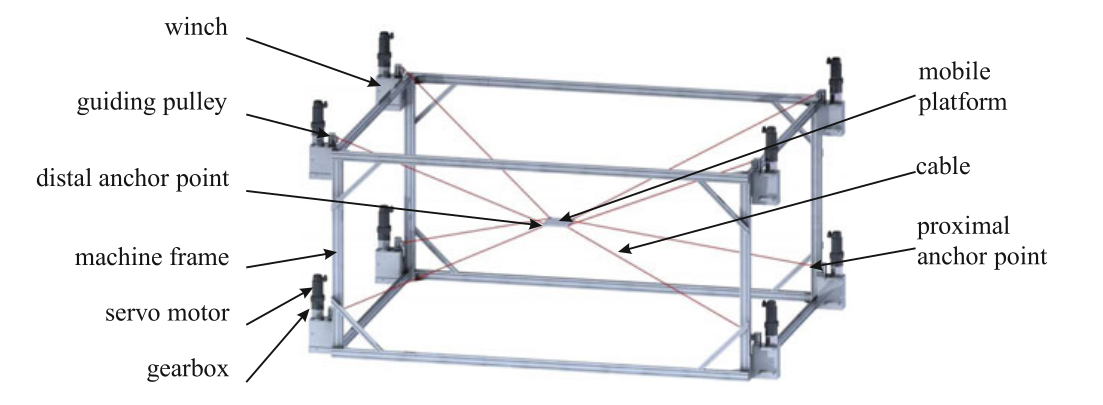
\includegraphics[width=0.5\textwidth]{Cabledrivenrobot.png}
\caption{A cable-driven robot from \cite{pott2018cable}.}
\label{fig:figure6}
\end{figure}

Cable-driven robots offer one main advantage over serial robots: they are light weight. This is because, unlike the serial case, the
motors do not have to bear the weight of other motors. Therefore, much higher speeds can be achieved. 

\section{Methodology}

\subsection{Inverse Kinematics Model}
Derivation for the inverse kinematics model.
Logic behind picking constant time over constant motor velocity.

\subsection{Planar Homography}

Since the camera does not have an overhead view of the workspace, the relationship $(x, y) = s(u, v)$ does not hold. Here
$(x, y)$ is the physical coordinate, $s$ is a scale factor, and $(u, v)$ is the pixel coordinate. There is a linear
relationship between the pixel coordinates and physical coordinates in plane described by a homography matrix. The homography
matrix is invertible, because unlike the general case where we a translating between a 3D point in space and a pixel in a 2D image,
we are translating between a 2D plane in reality and a 2D pixel space. The homography matrix has 8 degrees of freedom, $h_1, \dots, h_8$.

$$ H =
\begin{pmatrix}
h_1 & h_2 & h_3 \\
h_4 & h_5 & h_6 \\
h_7 & h_8 & 1 \\
\end{pmatrix}
$$

Let $X_1, X_2, X_3, X_4$ be four points on a physical plane in homogeneous coordinates and $x_1, x_2, x_3, x_4$ the corresponding pixel coordinates in homogeneous form.
Then the following equations

\begin{align*}
X_1 &= Hx_1 \\
X_2 &= Hx_2 \\
X_3 &= Hx_3 \\
X_4 &= Hx_4
\end{align*}

define a system of linear equations, which can be solved for $h_1, \dots, h_8$. This is why there is a calibration phase before the robot starts moving. Now
say there is a point on the video feed, $p$, whose physical coordinate is needed. Applying the homography matrix on the pixel coordinate, $P = Hp$, we get
$P$, the physical coordinate corresponding to $p$.

\subsection{Vision}
We used OpenCV for object tracking and everything related to computer vision. More specifically, we used OpenCV's CSRT
tracker. The figure below shows the control flow for the vision system.

\begin{figure}[h]
\centering
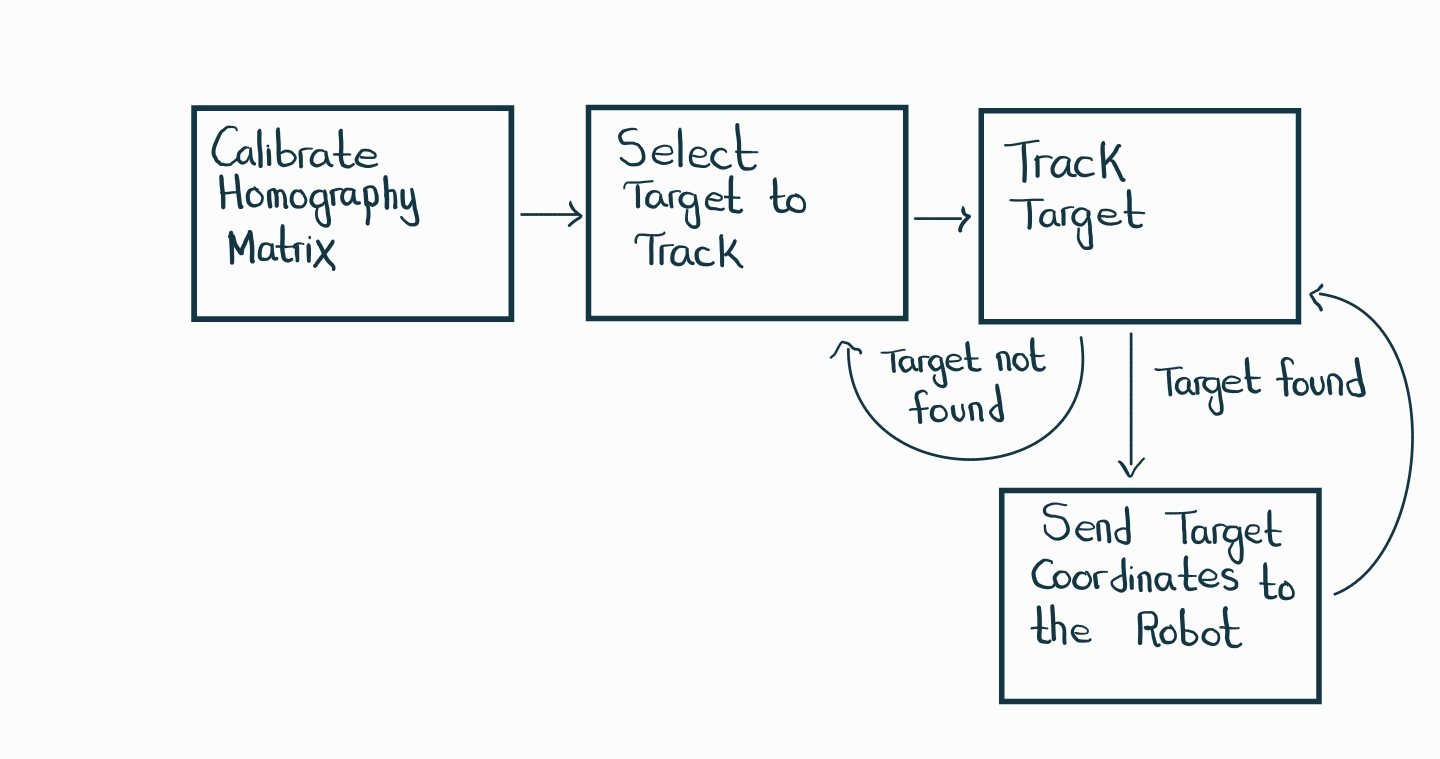
\includegraphics[width=0.5\textwidth]{VisionSystem.jpg}
\caption{Control flow for the vision system.}
\label{fig:figure4}
\end{figure}

First, marked points are selected in the video
feed to calibrate the homography matrix. Next, the user selects the target to be tracked. Depending on whether OpenCV
successfully tracks the object in the most recent frame, the path diverges into two. If the tracking fails, the user has
to select the target again. If the tracking is successful, the server sends the physical coordinates to the EV3 and continues
to track the target.

\section{Results}
Present your findings clearly using text, tables, and figures. Reference all figures and tables in the text.


\begin{figure}[h]
\centering
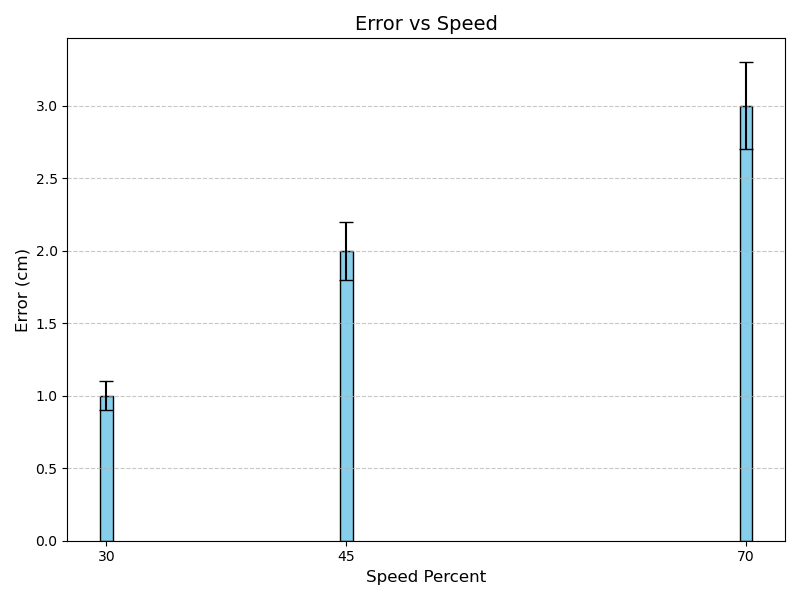
\includegraphics[width=0.6\textwidth]{TmpGraph.png}
\caption{A temporary error graph.}
\label{fig:figure5}
\end{figure}

\section{Discussion}
Analyze and interpret the results. Discuss their implications, limitations, and potential future work.
Could talk about why the end-effector could not be done here.
Remember to discuss the pulley problem. Using Lego connector pins as pulleys causes problems. We 3D printed pulleys
but they would slip. Limitations with the 3D printer precision. Also in the discussion should be why the error
values for the end-effector position are so low. Also should be talked about sources of error.
It's a planar robot, which means that it cannot exert force perpendicular to the plane. If weight is added to the end-effector
there is no way the robot can counteract that force. Which will cause the cables to bend. There is a mechanism we thought
about but did not have the time to implement. Compare the precision of the cable-driven robot with the lab2 robot arm that was
made using the same components. Another thing to include: why Broyden's method could not be used. If the jacobian is not
perfect, incorrect changes in the cable lengths would break the system.

\section{Conclusion}
Summarize the key findings and their significance. Suggest directions for further research (tension model?).


\bibliographystyle{plain}
\bibliography{references}

\appendix
\section{Appendix: Additional Details}
Code snippets that are important. Instructions on how to run the project (setting up srccpy and obsstudio).

\subsection{Instructions to Run the Project}


\end{document}
